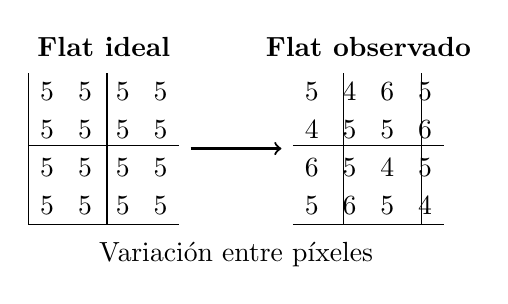
\begin{tikzpicture}[x=0.48cm,y=0.48cm]
  \node[font=\bfseries] at (2,4.7) {Flat ideal};
  \node[font=\bfseries] at (9,4.7) {Flat observado};
  \draw (0,0) grid (4,4);
  \draw (7,0) grid (11,4);
  \foreach \x in {0,...,3} {
    \foreach \y in {0,...,3} {
      \node at (\x+0.5,\y+0.5) {5};
    }
  }
  \node at (7.5,3.5) {5}; \node at (8.5,3.5) {4};
  \node at (9.5,3.5) {6}; \node at (10.5,3.5) {5};
  \node at (7.5,2.5) {4}; \node at (8.5,2.5) {5};
  \node at (9.5,2.5) {5}; \node at (10.5,2.5) {6};
  \node at (7.5,1.5) {6}; \node at (8.5,1.5) {5};
  \node at (9.5,1.5) {4}; \node at (10.5,1.5) {5};
  \node at (7.5,0.5) {5}; \node at (8.5,0.5) {6};
  \node at (9.5,0.5) {5}; \node at (10.5,0.5) {4};
  \draw[->,thick] (4.3,2) -- (6.7,2);
  \node[align=center] at (5.5,-0.8) {Variación entre píxeles};
\end{tikzpicture}